\documentclass[12pt] {article}
\usepackage{times}
\usepackage[margin=0.6in,bottom=1in,top=0.2in]{geometry}

\usepackage{hhline}
\usepackage{subfig}
\usepackage{graphicx}
\usepackage{amsmath}




\begin{document}

\title{Kronecker Product -  EEC289Q}
\author{Ahmed H. Mahmoud}
\date{February 8th, 2018}
\maketitle
%============Table========
%\begin{figure}[tbh]
% \centering    
%\begin{tabular}{ |p{4cm}|| p{2cm}|p{2cm}|p{2cm}|p{2cm}|}
% \hline
% & Processor 1 &  Processor 2  & Processor 3 & Processor 4\\ \hhline{|=|=|=|=|=|}
% \hline
% Performance          &$1.08$        &$1.425$       &\textbf{1.52}  &   \\
% \hline
%\end{tabular} 
%\caption{Metric table for the four processors}
%   \label{tab:metric}
%\end{figure} 
%============Figure========
%\begin{figure}[!tbh]
%\centering        
%   \subfloat {\includegraphics[width=0.65\textwidth]{fig2_4.png}}
%   \caption{ }
%   \label{fig:fig}
%\end{figure}

\paragraph{Analysis.} It is beneficial to start with a little analysis to figure if the problem is compute-bound or memory-bound in order to focus on the right optimization method. At first glance the problem seems memory-bound; for each output value we need to read two values and write one value while only doing one multiply operation. Thus, the arithmetic intensity can not exceed $1/3$. We quantified this by computing the \emph{Speed of Light}; the processing rate that can not be exceeded by assuming that the computation take no time and all memory access are fully coalesced and reside always at the top of the memory hierarchy. In order to carry out the Kronecker product of two matrices $A\in \mathcal{R}^{M\times M}$ and $B\in \mathcal{R}^{N\times N}$ to result into $C\in \mathcal{R}^{\left(M\times M \right)\times \left(N\times N\right)}$, we will need 
$
\underbrace{4M^{2}}_\text{Read $A$} + 
\underbrace{4N^{2}}_\text{Read $B$} +
\underbrace{4(NM)^{2}}_\text{Write $C$}
$
data movement while $(MN)^{2}$ FLOPS are needed. Figure ~\ref{fig:sol} shows the speed of light of different sizes of $A$ and $B$ (see caption) superimposed over the roofline of K40 device. The operation is severely memory-bound and only a very small fraction of peak performance (FLOPS) is achievable.  

\begin{figure}[!tbh]
\centering        
   \subfloat {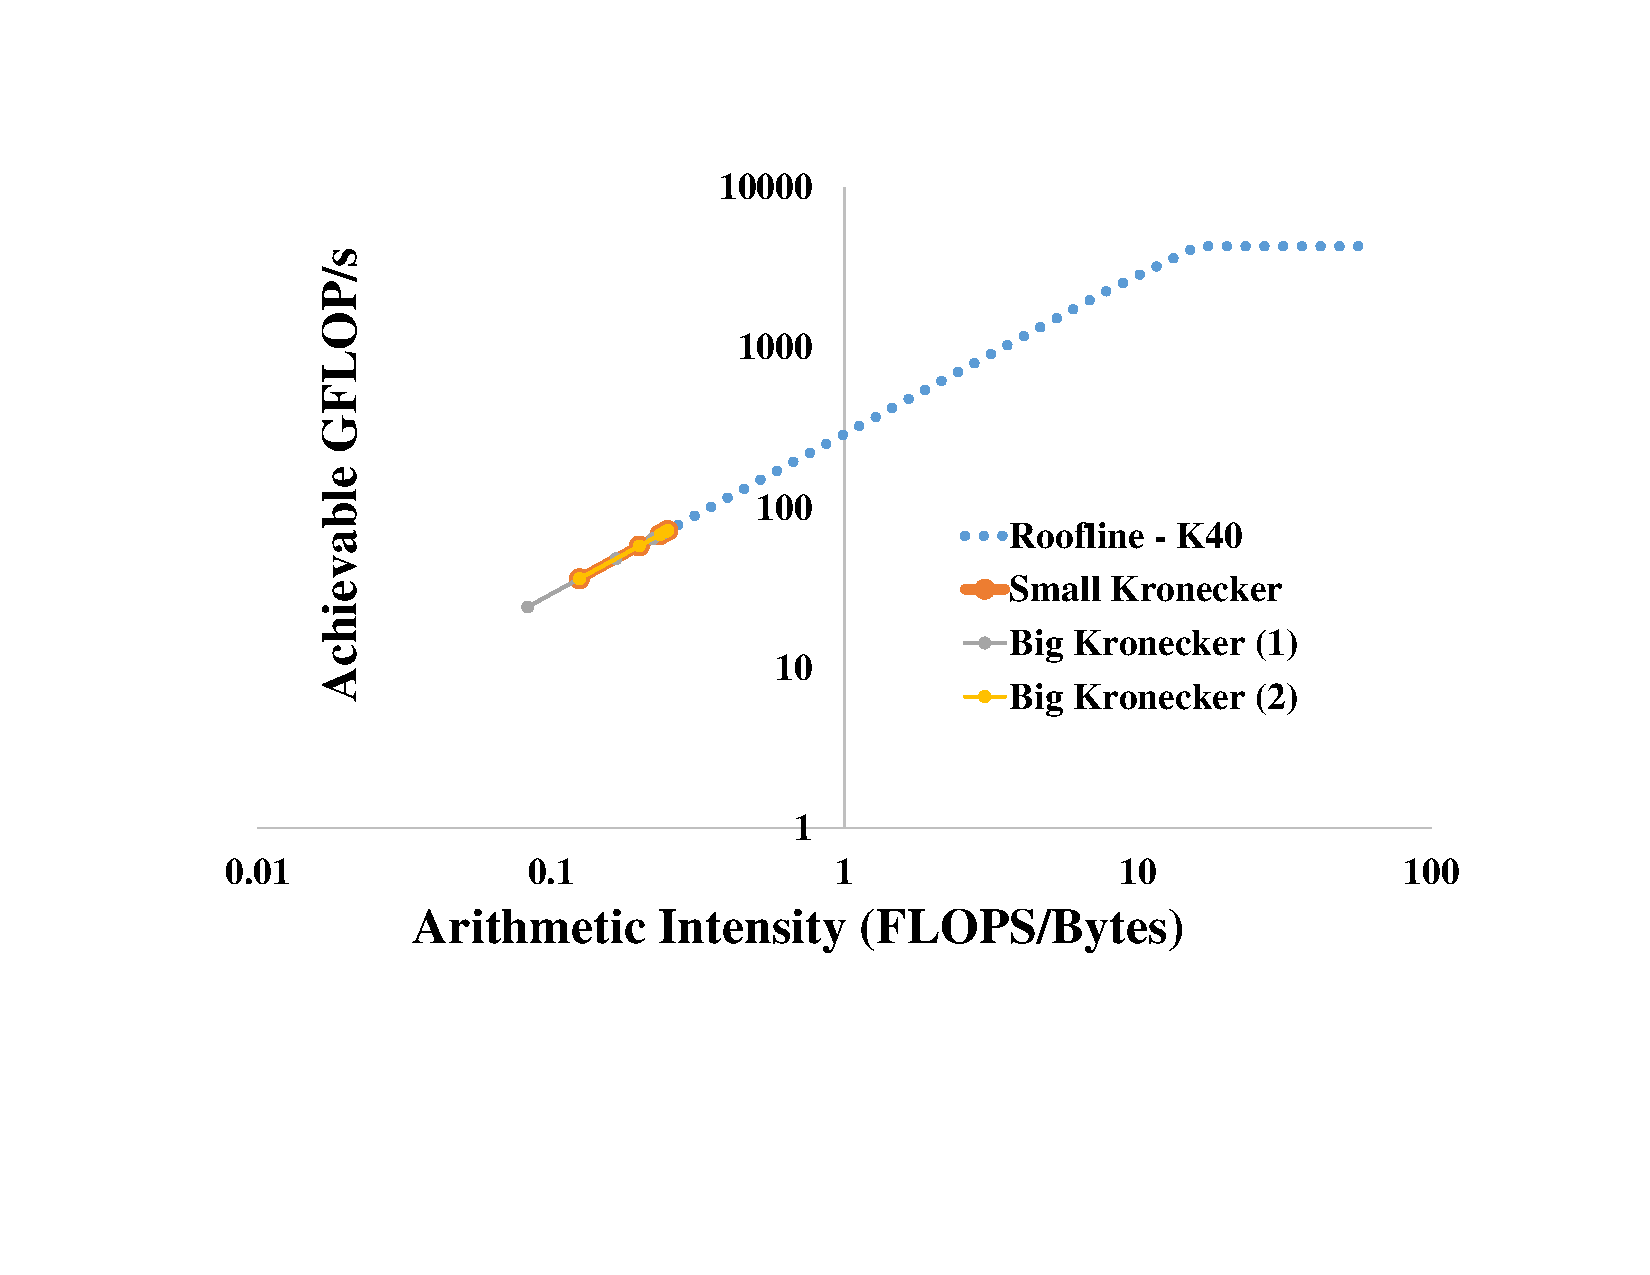
\includegraphics[width=0.5\textwidth]{fig/sol.pdf}}
   \caption{Speed of light of Kronecker product for three different configuration; Small Kronecker is for small $B$ and varying $A$ size, Big Kronecker (1) is for increasing $A$ and $B$ sizes at the same rate, while Big Kronecker (2) starts big $B$ and small $A$ and decreasing $B$ while increasing $A$.}   
   \label{fig:sol}
\end{figure}


\end{document}
